\documentclass[11pt,letterpaper]{article}
\usepackage[spanish,es-tabla]{babel}
\usepackage{fontspec}
\setmainfont{Liberation Serif}
\setmonofont{DejaVu Sans Mono}[Scale=0.78]
\usepackage{geometry}
\geometry{top=2.55cm,bottom=2.1cm,left=2.55cm,right=2.55cm,headheight=38pt,headsep=18pt}
\usepackage{graphicx}
\usepackage{array,longtable,ragged2e,colortbl}
\usepackage[table]{xcolor}
\usepackage{fancyhdr}
\usepackage{hyperref,xurl}
\usepackage{microtype}
\usepackage{enumitem}
\usepackage{fvextra}
\usepackage{needspace}
\usepackage{titlesec}
\usepackage{tocloft}
\usepackage{caption}
\usepackage{float}
\definecolor{azulPrimario}{HTML}{173D59}
\definecolor{azulSecundario}{HTML}{49768D}
\definecolor{grisTabla}{HTML}{E9EEF1}
\definecolor{grisBorde}{HTML}{BBC9CF}
\definecolor{grisCodigo}{HTML}{F4F6F8}
\hypersetup{colorlinks=true,linkcolor=azulPrimario,urlcolor=azulSecundario,bookmarksnumbered=true,pdftitle={Entrega 2 - Mandala Films},pdfauthor={Equipo ICN292}}
\emergencystretch=2em
\setlength{\parindent}{0pt}
\setlength{\parskip}{6.5pt plus 1pt minus 1pt}
\setlength{\LTpre}{8pt}
\setlength{\LTpost}{11pt}
\arrayrulecolor{grisBorde}
\pagestyle{fancy}
\fancyhf{}
\fancyhead[L]{
\includegraphics[height=0.65cm,keepaspectratio]{imagenes/image9.png}}
\fancyhead[R]{\textcolor{azulPrimario}{\footnotesize\textsc{Mandala Films \textbar\ Entrega 2}}}
\fancyfoot[C]{\thepage}
\renewcommand{\headrulewidth}{0pt}
\renewcommand{\footrulewidth}{0pt}
\fancypagestyle{portada}{%
  \fancyhf{}%
  \fancyhead[L]{
\includegraphics[height=0.65cm,keepaspectratio]{imagenes/image9.png}}%
  \fancyfoot[C]{\thepage}%
  \renewcommand{\headrulewidth}{0pt}%
}
\setcounter{secnumdepth}{3}
\setcounter{tocdepth}{3}
\renewcommand{\contentsname}{Índice de contenidos}
\titleformat{\section}[block]{\color{azulPrimario}\Large\bfseries}{\thesection.}{0.65em}{}[\vspace{1pt}\color{azulSecundario}\titlerule]
\titlespacing*{\section}{0pt}{19pt plus 2pt minus 2pt}{12pt}
\titleformat{\subsection}[block]{\color{azulPrimario}\large\bfseries}{\thesubsection}{0.75em}{}
\titlespacing*{\subsection}{0pt}{15pt plus 1pt minus 1pt}{6pt}
\titleformat{\subsubsection}[block]{\bfseries\normalsize}{\thesubsubsection}{0.65em}{}
\titlespacing*{\subsubsection}{0pt}{10pt}{5pt}
\renewcommand{\cftsecfont}{\bfseries\color{azulPrimario}}
\renewcommand{\cftsecpagefont}{\bfseries\color{azulPrimario}}
\renewcommand{\cftdotsep}{1.8}
\setlength{\cftbeforesecskip}{9pt}
\setlength{\cftbeforesubsecskip}{3pt}
\setlength{\cftbeforesubsubsecskip}{1pt}
\captionsetup{font=small,labelfont=bf,justification=centering,skip=4pt}
\DefineVerbatimEnvironment{SQL}{Verbatim}{breaklines=true,breakanywhere=true,fontsize=\footnotesize,frame=leftline,framesep=3mm,rulecolor=\color{grisBorde},bgcolor=grisCodigo}
\newcommand{\rotuloSQL}[1]{\par\noindent\textcolor{azulPrimario}{\bfseries #1}\par\vspace{-2pt}}
\begin{document}

% -------- PORTADA --------
\thispagestyle{portada}
\begin{minipage}[t]{0.78\textwidth}
  \centering
  \textbf{ICN292 - Sistemas de Información para la Gestión}\\[3pt]
  Segundo semestre 2026 / Campus Vitacura
\end{minipage}
\hfill
\begin{minipage}[t]{0.17\textwidth}
  \raggedleft
  
\includegraphics[width=2.45cm,keepaspectratio]{imagenes/image1.png}
\end{minipage}

\vspace*{2.4cm}
\begin{center}
  
\includegraphics[width=7.5cm]{imagenes/image2.jpg}

  \vspace{1.5cm}
  \textbf{Entrega 2 Proyecto}\\[3pt]
  \textbf{Mandala Films}
\end{center}
\vfill

\textbf{Integrantes:}\\
Agustin Barnils --- 202360650-2\\
Paula Daroch --- 202266510-6\\
Catalina Jofre --- 202360507-7\\
Antar Pizarro --- 202260576-6\\
Antonella Dagnino --- 202210025-7

\textbf{Profesores:} Patricio Eduardo Cifuentes Rey, José Luis Sáez Tamayo

\textbf{Repositorio:} \url{https://github.com/abarnils/ICN292-Mandala-Films}

\vspace*{1.25cm}
\clearpage
\pdfbookmark[1]{Índice de contenidos}{indice}
\tableofcontents
\clearpage
% -------- INFORME: contenido íntegro con jerarquía de títulos --------


\needspace{5\baselineskip}\section{Resumen ejecutivo}

Mandala Films presenta actualmente un problema de gestión asociado al seguimiento de sus proyectos audiovisuales, ya que la información se encuentra distribuida entre planillas de Excel, calendarios, correos electrónicos, WhatsApp, notas y pizarras. Esta forma de trabajo dificulta conocer rápidamente el estado de cada proyecto y sus costos asociados, lo que genera pérdida de tiempo y desgaste operacional. A partir de este problema, se propuso un Sistema de Información para la Gestión, orientado a centralizar el seguimiento de proyectos, etapas, gastos, honorarios y resultados financieros.


En la Entrega 2 se avanzó desde el diseño preliminar desarrollado en la Entrega 1 hacia componentes concretos de la solución. El modelo entidad-relación fue revisado y normalizado a tercera forma normal (3FN), incorporando catálogos, claves foráneas, reglas de integridad y ajustes destinados a reducir redundancias e inconsistencias. También se desarrollaron datos sintéticos y consultas SQL orientadas al análisis de proyectos, la participación y los honorarios de los trabajadores, y los resultados económicos por período.


Además, se implementó en n8n una automatización asociada al control de sobrecostos definido en el RF04. El flujo recibe gastos, calcula el porcentaje ejecutado del presupuesto y clasifica los casos para generar alertas cuando corresponde. Las pruebas permitieron comprobar el comportamiento esperado en la mayoría de los casos e identificar fallas relacionadas con datos incompletos, validaciones previas y envíos simultáneos.


Como resultado, la Entrega 2 permite validar de manera más concreta la propuesta definida inicialmente y detectar aspectos que todavía requieren integración. La solución mantiene decisiones relevantes del caso, como conservar manualmente los cambios de etapa del proyecto, y evidencia que la automatización y el modelo de datos deben mantenerse alineados con la forma real de trabajo de la empresa. Entre las principales limitaciones se encuentra que algunos componentes siguen funcionando por separado y con datos sintéticos, por lo que una implementación completa requeriría integrar la automatización, la base de datos y los mecanismos de notificación en un mismo sistema.


\clearpage
\needspace{5\baselineskip}\section{Automatización del control de sobrecosto}


\needspace{6\baselineskip}\subsection{Criterios y funcionamiento de la automatización}

Se automatizó el control de sobrecostos del BPMN to-be. Cuando se ingresa un gasto variable, el flujo calcula el porcentaje del presupuesto ya ejecutado mediante la fórmula (gasto acumulado + monto) / presupuesto aprobado $\times$ 100, y lo clasifica en cuatro estados: INVALIDO (presupuesto o monto menores o iguales a 0), SUPERADO (desde el 100 \%), CERCA (desde el 80 \%) y OK. El umbral del 80 \% fue propuesto por el equipo y validado por el dueño. En los estados CERCA y SUPERADO se envía una notificación, y cada decisión queda registrada en una hoja de Google Sheets. Esto responde al RF04 y al problema de la pérdida de registro de montos en gastos como bencina y arriendos. Los cambios de etapa y la evaluación del sobrecosto siguen siendo manuales, porque el dueño pidió ingresarlos de esa manera.


\needspace{6\baselineskip}\subsection{Implementación y casos de prueba}

La solución consta de dos workflows en n8n. El emisor simula al SIG, que todavía no existe: genera siete gastos de prueba y los envía de uno en uno, cada 3 segundos, al webhook. El flujo de sobrecostos los recibe, calcula el porcentaje, los clasifica mediante un Switch, asigna el estado y el mensaje, notifica, registra y responde al emisor. Se probó con siete casos sintéticos (S01 a S07) utilizando la Production URL. Seis se clasificaron como se esperaba y quedaron registrados en la hoja; además, llegaron tres notificaciones (CERCA al 80 \% y dos casos SUPERADO, al 100 \% y al 110 \%).


\needspace{6\baselineskip}\subsection{Fallas detectadas y limitaciones}

Las pruebas también evidenciaron fallas, que fueron documentadas. El caso S07, correspondiente a un gasto sin el dato de gasto acumulado, falla en el cálculo y no deja registro ni alerta. El flujo calcula antes de validar, por lo que, con presupuesto 0, el porcentaje queda vacío y, con un monto negativo, el resultado pierde sentido. Además, al enviar los siete casos simultáneamente se perdían filas en la hoja; al enviarlos de uno en uno, cada 3 segundos, se registraron las seis filas esperadas. Entre las limitaciones, el gasto llega con el presupuesto y el acumulado ya incluidos, la notificación se dirige a un webhook de prueba en lugar de Administración y Finanzas, y el registro se realiza en Google Sheets en vez de la base de datos del modelo.


\needspace{5\baselineskip}\subsection{Relación entre los nodos de n8n y el BPMN to-be}

\begingroup
\footnotesize
\setlength{\tabcolsep}{3.0pt}
\renewcommand{\arraystretch}{1.17}
\begin{longtable}{|>{\RaggedRight\arraybackslash}p{0.29\linewidth}|>{\RaggedRight\arraybackslash}p{0.29\linewidth}|>{\RaggedRight\arraybackslash}p{0.35\linewidth}|}
\hline
\rowcolor{grisTabla}
\textbf{Nodo en n8n} & \textbf{Tarea del BPMN to-be} & \textbf{Qué hace} \\ \hline
\endfirsthead
\hline
\rowcolor{grisTabla}
\textbf{Nodo en n8n} & \textbf{Tarea del BPMN to-be} & \textbf{Qué hace} \\ \hline
\endhead
\hline
\endfoot
Emisor (Trigger manual, Code, HTTP Request) y Webhook & Ingresar gastos variables ejecutados al SIG & Envía y recibe el gasto con proyecto, categoría, monto, presupuesto y acumulado \\ \hline
Edit Fields (porcentaje) y Switch & Gateway ¿Gastos ejecutados cerca o superiores al presupuesto? & Calcula el porcentaje y clasifica en INVALIDO, SUPERADO, CERCA u OK \\ \hline
HTTP Request (webhook.site) & Enviar alerta de sobrecosto & Notifica solo en CERCA y SUPERADO \\ \hline
Google Sheets (registro) y Respond to Webhook & Sin tarea propia & Guarda cada decisión como rastro y responde al emisor \\ \hline
\end{longtable}
\endgroup


\needspace{5\baselineskip}\section{Modelo entidad-relación en 3FN}

\needspace{5\baselineskip}\subsection{Diagrama entidad-relación}

\begin{center}
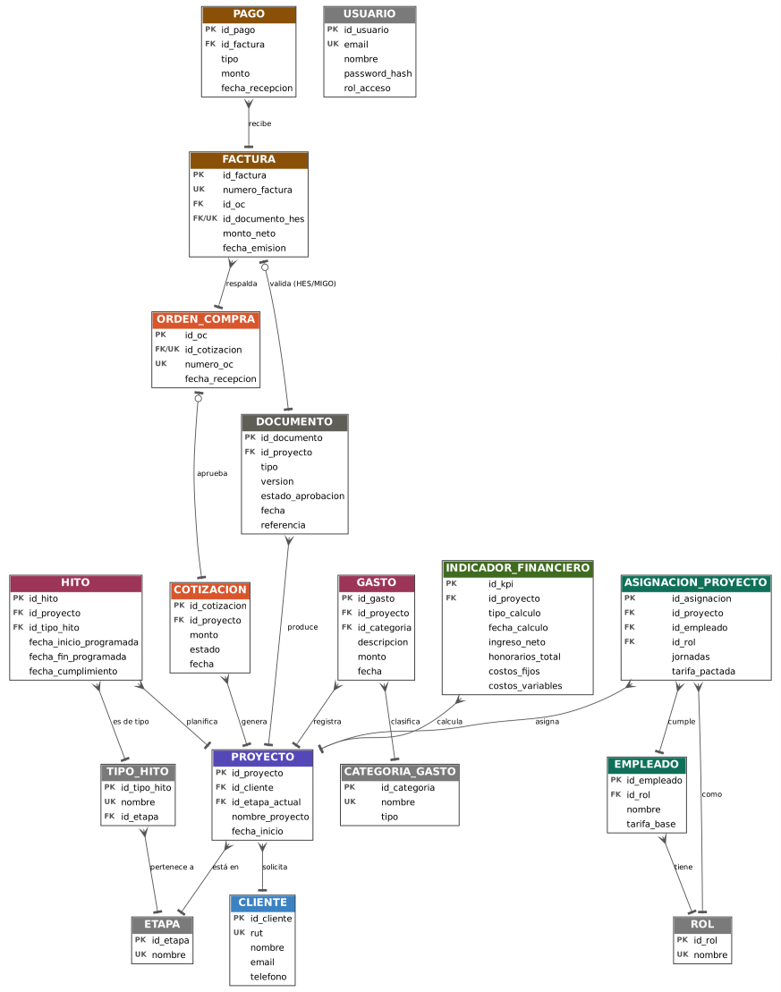
\includegraphics[height=17.0cm,width=\linewidth,keepaspectratio]{imagenes/image3.png}\captionof{figure}{Diagrama entidad-relación del modelo normalizado a 3FN.}
\end{center}


\clearpage
\needspace{4\baselineskip}\subsection{Cambios respecto del modelo preliminar}

La tabla siguiente resume qué se modificó respecto de la Entrega 1 y por qué. Las tablas ORDEN\_COMPRA y DOCUMENTO se mantuvieron sin cambios de fondo, al igual que las relaciones principales entre cliente, proyecto, cotización, orden de compra, factura y pago.


\begingroup
\footnotesize
\setlength{\tabcolsep}{3.0pt}
\renewcommand{\arraystretch}{1.17}
\begin{longtable}{|>{\RaggedRight\arraybackslash}p{0.055\linewidth}|>{\RaggedRight\arraybackslash}p{0.21\linewidth}|>{\RaggedRight\arraybackslash}p{0.09\linewidth}|>{\RaggedRight\arraybackslash}p{0.26\linewidth}|>{\RaggedRight\arraybackslash}p{0.3\linewidth}|}
\hline
\rowcolor{grisTabla}
\textbf{N.º} & \textbf{Elemento de la E1} & \textbf{Criterio} & \textbf{Problema} & \textbf{Solución} \\ \hline
\endfirsthead
\hline
\rowcolor{grisTabla}
\textbf{N.º} & \textbf{Elemento de la E1} & \textbf{Criterio} & \textbf{Problema} & \textbf{Solución} \\ \hline
\endhead
\hline
\endfoot
1 & CLIENTE.contacto & 1FN & Atributo compuesto (correo + teléfono en un campo). & Se separa en email y teléfono. \\ \hline
2 & \path{PROYECTO.presupuesto_aprobado} & 3FN & Repite el monto de la cotización aprobada: al cambiar uno había que actualizar el otro. & Se elimina. El presupuesto es el monto de la cotización APROBADA (índice único parcial) y se consulta en \path{v_presupuesto_proyecto}. \\ \hline
3 & \path{PROYECTO.estado_actual} & Dominio & Texto libre: permite etapas mal escritas. & Pasa a id\_etapa\_actual (FK a ETAPA). Se agrega la etapa inicial «Cotización», porque el proyecto existe antes de aceptarse la cotización. \\ \hline
4 & EMPLEADO.rol y \path{ASIGNACION.rol_en_proyecto} & Dominio & Texto libre con variantes de escritura. & Catálogo ROL; ambas columnas pasan a ser FK. \\ \hline
5 & \path{ASIGNACION.honorario_calculado} & 3FN & Valor derivado (tarifa $\times$ tiempo) guardado como dato. & Se reemplaza por jornadas y tarifa\_pactada; el honorario se calcula en \path{v_asignacion_honorario}. \\ \hline
6 & HITO.etapa y HITO.estado & 3FN & La etapa depende del tipo de hito, y el estado se deduce de las fechas. & Catálogo TIPO\_HITO (que trae la etapa). El estado se calcula en v\_hito\_estado. La fecha programada pasa a inicio y fin para poder dibujar la Gantt (RF07). \\ \hline
7 & GASTO.tipo y GASTO.categoria & 3FN & La categoría determina el tipo (bencina $\rightarrow$ variable): dependencia transitiva. & Catálogo CATEGORIA\_GASTO (con tipo); GASTO guarda solo id\_categoria. \\ \hline
8 & \path{FACTURA.id_proyecto} & 3FN & Ya se obtiene vía OC $\rightarrow$ cotización $\rightarrow$ proyecto; guardarlo permitía facturas que contradicen su OC. & Se elimina. El proyecto se obtiene en v\_factura y un trigger valida que OC y HES/MIGO sean del mismo proyecto. \\ \hline
9 & FACTURA.iva & 3FN & Depende de monto\_neto (IVA = 19 \% del neto). & Se elimina; v\_factura calcula IVA, total, pagado y saldo. \\ \hline
10 & \path{INDICADOR_FINANCIERO.iva}, ebitda, margen & 3FN & Se calculan a partir de otros atributos de la misma fila. & Se guardan solo los insumos congelados (ingreso, honorarios, costos); los derivados salen de \path{v_indicador_financiero}. \\ \hline
11 & (no existía) USUARIO & Cobertura & La E1 pide autenticación (RNF02) y menciona una tabla de usuarios, pero el ER no la tenía. & Se agrega USUARIO. \\ \hline
12 & (no existía) PAGO.tipo, \path{FACTURA.numero_factura} & Cobertura & La E1 dice «anticipo + pago final» y el flujo usa el folio de facturacion.cl, pero no había atributo. & Se agregan tipo y numero\_factura. \\ \hline
\end{longtable}
\endgroup


\needspace{4\baselineskip}\subsection{Verificación de normalización}

\begin{itemize}[leftmargin=1.5em,itemsep=2pt,topsep=3pt]

\item 1FN: todos los atributos son atómicos (se separó «contacto» en email y teléfono) y cada tabla tiene clave primaria.

\item 2FN: todas las claves primarias son de una sola columna, por lo que ningún atributo puede depender de solo una parte de la clave.

\item 3FN: en cada tabla los únicos determinantes son claves candidatas; ningún atributo no clave depende de otro atributo no clave.

\end{itemize}

Hay una excepción consciente: INDICADOR\_FINANCIERO guarda ingresos, honorarios y costos, que podrían recalcularse. Se conservan como una fotografía histórica, porque el indicador estimado se fija al aceptar la cotización, antes de que existan asignaciones y gastos, y no debe cambiar después. Los valores derivados de esa fotografía (IVA, EBITDA y margen) sí se calculan mediante una vista.


\needspace{4\baselineskip}\subsection{Anomalías que el modelo evita}

\begin{itemize}[leftmargin=1.5em,itemsep=2pt,topsep=3pt]

\item Actualización: En la E1, cambiar el monto de una cotización aprobada obligaba a actualizar también PROYECTO.presupuesto\_aprobado; si se olvidaba, el sistema mostraba dos presupuestos distintos. Ahora el monto existe en un solo lugar.

\item Actualización: En la E1, una factura podía declarar un proyecto distinto al de su OC. Ahora el proyecto no se almacena en FACTURA y un trigger impide mezclar una OC y un HES/MIGO de proyectos diferentes.

\item Inserción: En la E1 no se podía registrar una categoría de gasto nueva (p. ej., «Catering») sin tener ya un gasto de esa categoría. Con los catálogos ROL, CATEGORIA\_GASTO y TIPO\_HITO, las categorías pueden crearse por separado.

\item Eliminación: En la E1, al borrar el único gasto de bencina se perdía el registro de que «bencina» es un gasto variable. Ahora ese dato se conserva en CATEGORIA\_GASTO.

\item Inconsistencia: Con roles y estados como texto libre, aparecían variantes («Camarógrafo», «camarografo», «camarógrafo »). Los catálogos y las restricciones CHECK lo impiden.

\end{itemize}


\needspace{4\baselineskip}\subsection{Diccionario de datos}

La tabla siguiente muestra, por entidad, la clave primaria, las claves foráneas y los demás atributos. El detalle completo (tipo de dato, nulidad y regla de cada atributo) se encuentra en el archivo docs/03-modelo-datos.md del repositorio.


\begingroup
\footnotesize
\setlength{\tabcolsep}{3.0pt}
\renewcommand{\arraystretch}{1.17}
\begin{longtable}{|>{\RaggedRight\arraybackslash}p{0.245\linewidth}|>{\RaggedRight\arraybackslash}p{0.14\linewidth}|>{\RaggedRight\arraybackslash}p{0.26\linewidth}|>{\RaggedRight\arraybackslash}p{0.285\linewidth}|}
\hline
\rowcolor{grisTabla}
\textbf{Tabla} & \textbf{PK} & \textbf{FK} & \textbf{Otros atributos} \\ \hline
\endfirsthead
\hline
\rowcolor{grisTabla}
\textbf{Tabla} & \textbf{PK} & \textbf{FK} & \textbf{Otros atributos} \\ \hline
\endhead
\hline
\endfoot
CLIENTE & id\_cliente & — & rut (UK), nombre, email, telefono \\ \hline
PROYECTO & id\_proyecto & id\_cliente $\rightarrow$ cliente; id\_etapa\_actual $\rightarrow$ etapa & nombre\_proyecto (UK compuesta), fecha\_inicio \\ \hline
ETAPA & id\_etapa & — & nombre (UK) \\ \hline
COTIZACION & id\_cotizacion & id\_proyecto $\rightarrow$ proyecto & monto, estado, fecha \\ \hline
ORDEN\_COMPRA & id\_oc & id\_cotizacion $\rightarrow$ cotizacion (UK) & numero\_oc (UK), fecha\_recepcion \\ \hline
EMPLEADO & id\_empleado & id\_rol $\rightarrow$ rol & nombre, tarifa\_base \\ \hline
ROL & id\_rol & — & nombre (UK) \\ \hline
\path{ASIGNACION_PROYECTO} & id\_asignacion & id\_proyecto $\rightarrow$ proyecto; id\_empleado $\rightarrow$ empleado; id\_rol $\rightarrow$ rol & jornadas, tarifa\_pactada \\ \hline
HITO & id\_hito & id\_proyecto $\rightarrow$ proyecto; id\_tipo\_hito $\rightarrow$ tipo\_hito & \path{fecha_inicio_programada}, \path{fecha_fin_programada}, \path{fecha_cumplimiento} \\ \hline
TIPO\_HITO & id\_tipo\_hito & id\_etapa $\rightarrow$ etapa & nombre (UK) \\ \hline
GASTO & id\_gasto & id\_proyecto $\rightarrow$ proyecto; id\_categoria $\rightarrow$ categoria\_gasto & descripcion, monto, fecha \\ \hline
CATEGORIA\_GASTO & id\_categoria & — & nombre (UK), tipo \\ \hline
DOCUMENTO & id\_documento & id\_proyecto $\rightarrow$ proyecto & tipo, version, estado\_aprobacion, fecha, referencia \\ \hline
FACTURA & id\_factura & id\_oc $\rightarrow$ orden\_compra; id\_documento\_hes $\rightarrow$ documento (UK) & numero\_factura (UK), monto\_neto, fecha\_emision \\ \hline
PAGO & id\_pago & id\_factura $\rightarrow$ factura & tipo, monto, fecha\_recepcion \\ \hline
\path{INDICADOR_FINANCIERO} & id\_kpi & id\_proyecto $\rightarrow$ proyecto & tipo\_calculo, fecha\_calculo, ingreso\_neto, honorarios\_total, costos\_fijos, costos\_variables \\ \hline
USUARIO & id\_usuario & — & nombre, email (UK), password\_hash, rol\_acceso \\ \hline
\end{longtable}
\endgroup


\needspace{4\baselineskip}\subsection{Reglas de integridad}

Las reglas se aplican en la base de datos cuando es posible (mediante restricciones, CHECK y triggers), y en el backend cuando dependen del flujo de la aplicación.


\begingroup
\footnotesize
\setlength{\tabcolsep}{3.0pt}
\renewcommand{\arraystretch}{1.17}
\begin{longtable}{|>{\RaggedRight\arraybackslash}p{0.065\linewidth}|>{\RaggedRight\arraybackslash}p{0.64\linewidth}|>{\RaggedRight\arraybackslash}p{0.23\linewidth}|}
\hline
\rowcolor{grisTabla}
\textbf{ID} & \textbf{Regla} & \textbf{Dónde se aplica} \\ \hline
\endfirsthead
\hline
\rowcolor{grisTabla}
\textbf{ID} & \textbf{Regla} & \textbf{Dónde se aplica} \\ \hline
\endhead
\hline
\endfoot
R01 & Un proyecto tiene como máximo una cotización aprobada (su presupuesto). & BD: índice único parcial \\ \hline
R02 & Una OC solo existe si su cotización está APROBADA. & BD: trigger \\ \hline
R03 & Una cotización tiene como máximo una OC. & BD: UNIQUE \\ \hline
R04 & Una factura exige OC y un HES/MIGO APROBADO del mismo proyecto. & BD: NOT NULL + trigger \\ \hline
R05 & Un HES/MIGO respalda como máximo una factura. & BD: UNIQUE \\ \hline
R06 & Los montos, jornadas y versiones son positivos; las fechas de término son posteriores o iguales a las de inicio. & BD: CHECK \\ \hline
R07 & El RUT del cliente es único y tiene formato válido. & BD: UNIQUE + CHECK (dígito verificador: backend) \\ \hline
R08 & Un empleado no repite el mismo rol en el mismo proyecto. & BD: UNIQUE \\ \hline
R09 & Un proyecto tiene como máximo un indicador ESTIMADO y uno REAL. & BD: UNIQUE \\ \hline
R10 & No se borran registros que tengan dependientes (cliente con proyectos, etc.). & BD: FK sin cascada \\ \hline
R11 & Las etapas, estados y tipos solo admiten los valores del dominio. & BD: FK a catálogo o CHECK \\ \hline
R12 & El avance de etapa lo confirma manualmente el productor. & Backend \\ \hline
R13 & Al aceptar la cotización se crea el indicador ESTIMADO; al cierre, el REAL. & Backend \\ \hline
R14 & La suma de pagos no debe superar el total de la factura. & Backend (v\_factura.saldo permite detectarlo) \\ \hline
R15 & Alerta de sobrecosto cuando el gasto llega al 90 \% del presupuesto. & Vista \path{v_presupuesto_proyecto} (umbral supuesto) \\ \hline
R16 & Solo DUENO y ADMIN\_FINANZAS acceden al sistema. & BD: CHECK + backend \\ \hline
\end{longtable}
\endgroup


\needspace{4\baselineskip}\subsection{Implementación y verificación}

El archivo schema.sql se ejecutó sobre una base vacía de PostgreSQL 16, dos veces consecutivas y sin errores, y crea 17 tablas y 5 vistas. Con datos de prueba mínimos se comprobó, además, que la base acepta los casos válidos y rechaza siete casos inválidos: una segunda cotización aprobada para un proyecto, una orden de compra sobre una cotización no aprobada, una factura respaldada por un documento que no es HES/MIGO, una factura con un HES de otro proyecto, un RUT duplicado, un monto negativo y la eliminación de un cliente que tiene proyectos. Los datos de prueba definitivos se encuentran en seed.sql.


\needspace{5\baselineskip}\subsection{Supuestos del modelo}

(1) el proyecto nace en la etapa «Cotización» y pasa a Preproducción al aceptarse la cotización, porque la cotización depende del proyecto; (2) la tarifa base es propia de cada empleado, no del rol; (3) la alerta de sobrecosto compara el gasto con el monto de la cotización aprobada y se activa desde el 90 \%; (4) el IVA es del 19 \% y los montos están expresados en pesos chilenos sin decimales.


\needspace{5\baselineskip}\section{Base de datos y consultas SQL}

\needspace{5\baselineskip}\subsection{Estructura de la base de datos}

A partir de la información recopilada en la entrevista y del sistema de registro que utiliza actualmente la empresa, se generó una base de datos que mantiene su estructura de trabajo habitual, pero reorganiza la información de manera más eficiente para su tratamiento. Para ello, se crearon cuatro tablas. La primera corresponde a proyectos y registra el nombre de cada proyecto, el ejecutivo encargado, las fechas de inicio y término tentativas y una serie de variables booleanas que permiten marcar los procesos completados. La segunda tabla registra a los trabajadores de la empresa, con su nombre y RUT. La tercera, llamada «honorarios», relaciona las dos tablas anteriores, lo que permite identificar a los trabajadores asignados a cada proyecto, los honorarios asociados a su participación y si el pago correspondiente fue realizado. La cuarta y última tabla corresponde a los costos fijos, donde se registran los diferentes costos mensuales asociados al funcionamiento de la empresa.


\rotuloSQL{Código SQL: creación de la base de datos y sus tablas}
\begin{SQL}
DROP DATABASE IF EXISTS mandalafilms;
CREATE DATABASE mandalafilms;
USE mandalafilms;

CREATE TABLE proyectos (
id_proyecto INT AUTO_INCREMENT,
nombre_proyecto VARCHAR(100) NOT NULL,
ejecutivo VARCHAR(120) NOT NULL,
fecha_inicio DATE,
fecha_termino DATE,
presupuesto DECIMAL(10,2) NOT NULL,
contacto BOOLEAN NOT NULL DEFAULT FALSE,
visita BOOLEAN NOT NULL DEFAULT FALSE,
guion BOOLEAN NOT NULL DEFAULT FALSE,
grabacion BOOLEAN NOT NULL DEFAULT FALSE,
locucion BOOLEAN NOT NULL DEFAULT FALSE,
edicion_offline BOOLEAN NOT NULL DEFAULT FALSE,
animacion BOOLEAN NOT NULL DEFAULT FALSE,
edicion_online BOOLEAN NOT NULL DEFAULT FALSE,
color BOOLEAN NOT NULL DEFAULT FALSE,
entrega BOOLEAN NOT NULL DEFAULT FALSE,
oc BOOLEAN NOT NULL DEFAULT FALSE,
factura BOOLEAN NOT NULL DEFAULT FALSE,
pago BOOLEAN NOT NULL DEFAULT FALSE,
PRIMARY KEY (id_proyecto)
);

CREATE TABLE trabajadores (
id_trabajador INT AUTO_INCREMENT,
nombre_trabajador VARCHAR(100) NOT NULL,
rut VARCHAR(15) NOT NULL,
PRIMARY KEY (id_trabajador)
);

CREATE TABLE honorarios (
id_honorario INT AUTO_INCREMENT,
id_proyecto INT NOT NULL,
id_trabajador INT NOT NULL,
rol VARCHAR(120),
honorario_bruto DECIMAL(10,2) NOT NULL,
boleta BOOLEAN NOT NULL DEFAULT FALSE,
pagado BOOLEAN NOT NULL DEFAULT FALSE,
PRIMARY KEY (id_honorario),
FOREIGN KEY (id_proyecto) REFERENCES proyectos(id_proyecto),
FOREIGN KEY (id_trabajador) REFERENCES trabajadores(id_trabajador)
);

CREATE TABLE costos_fijos (
id_costo INT AUTO_INCREMENT,
nombre_costo VARCHAR(80),
costo DECIMAL(10,2),
PRIMARY KEY (id_costo)
);
\end{SQL}


\needspace{5\baselineskip}\subsection{Datos sintéticos de prueba}

Una vez definida la estructura, se generaron datos sintéticos para ejecutar consultas y observar el funcionamiento del sistema. En concreto, se crearon 10 trabajadores, 3 proyectos, 12 asignaciones de trabajadores a proyectos y 4 tipos de costos fijos, que se incorporaron a la base mediante el siguiente código:


\rotuloSQL{Código SQL: inserción de datos sintéticos}
\begin{SQL}
USE mandalafilms;

INSERT INTO trabajadores (nombre_trabajador, rut) VALUES
('Camila Rojas', '17482910-3'),
('Mateo Sepúlveda', '16938471-K'),
('Javiera Soto', '18204955-2'),
('Sebastián Contreras', '15847291-8'),
('Valentina Núñez', '19048273-6'),
('Diego Morales', '14739204-5'),
('Fernanda Espinoza', '18651029-1'),
('Tomás Herrera', '17192834-9'),
('Catalina Fuentes', '19384712-4'),
('Nicolás Castro', '16294817-7');

INSERT INTO proyectos (
nombre_proyecto, ejecutivo, fecha_inicio, fecha_termino, presupuesto, contacto, visita, guion, grabacion, locucion, edicion_offline, animacion, edicion_online, color, entrega, oc, factura, pago ) VALUES
('Campaña Bebida Botánica', 'Andrés Valdés', '2026-11-10', '2026-12-15', 4500000.00, TRUE, TRUE, TRUE, FALSE, FALSE, FALSE, FALSE, FALSE, FALSE, FALSE, FALSE, FALSE, FALSE),
('Documental Ruta del Sur', 'Paula Mardones', '2026-09-01', '2026-11-30', 8200000.00, TRUE, TRUE, TRUE, TRUE, TRUE, TRUE, TRUE, FALSE, FALSE, FALSE, TRUE, TRUE, FALSE ),
('Spot Lanzamiento EcoTech', 'Andrés Valdés', '2026-07-15', '2026-09-20', 6100000.00, TRUE, TRUE, TRUE, TRUE, TRUE, TRUE, TRUE, TRUE, TRUE, TRUE, TRUE, TRUE, TRUE );

INSERT INTO honorarios (id_proyecto, id_trabajador, rol, honorario_bruto, boleta, pagado) VALUES
(1, 2, 'camarografo',  480000.00, TRUE,  FALSE),
(1, 5, 'asistente',    320000.00, FALSE, FALSE),
(1, 8, 'editor',       610000.00, FALSE, FALSE),
(2, 1, 'camarografo', 1450000.00, TRUE,  TRUE),
(2, 3, 'editor',       890000.00, TRUE,  FALSE),
(2, 4, 'sonidista',    740000.00, TRUE,  TRUE),
(2, 7, 'asistente',    530000.00, FALSE, FALSE),
(2, 10, 'colorista',   680000.00, TRUE,  FALSE),
(3, 1, 'camarografo', 1200000.00, TRUE,  TRUE),
(3, 6, 'editor',       950000.00, TRUE,  TRUE),
(3, 8, 'animador',     560000.00, TRUE,  TRUE),
(3, 9, 'asistente',    790000.00, TRUE,  TRUE);

INSERT INTO costos_fijos (nombre_costo, costo) VALUES
('arriendo', 750000.00),
('sueldo', 1200000.00),
('creditos', 400000.00),
('telefonia', 50000.00);
\end{SQL}


\needspace{5\baselineskip}\subsection{Consultas de negocio en SQL}

Luego de construir la base de datos, se realizaron tres consultas relevantes. Para ello, se consideraron el funcionamiento descrito y las preferencias de la empresa, que manifestó especial interés en la automatización del sistema de costos.


\needspace{5\baselineskip}\subsubsection{Consulta 1: seguimiento y rentabilidad de un proyecto}

La primera es una consulta compuesta que permite observar el estado de un proyecto específico, los trabajadores asignados, los costos relacionados y las ganancias. Para ejecutarla, se debe seleccionar el nombre del proyecto de interés y el valor de los costos variables de producción, que dependen de cada proyecto y no siguen un criterio único estandarizable. Se destacan los campos que deben modificarse en cada consulta.


\rotuloSQL{Código SQL: seguimiento de un proyecto}
\begin{SQL}
USE mandalafilms;

SET @nombre_proyecto = 'Documental Ruta del Sur';
SET @costos_produccion = 350000;

SELECT *
FROM proyectos
WHERE nombre_proyecto = @nombre_proyecto;

SELECT
h.rol AS equipo,
t.nombre_trabajador as trabajador,
h.honorario_bruto AS honorario_bruto,
h.honorario_bruto* 1.145 AS honorario_liquido
FROM trabajadores t
JOIN honorarios h ON t.id_trabajador = h.id_trabajador
JOIN proyectos p ON h.id_proyecto = p.id_proyecto
WHERE p.nombre_proyecto = @nombre_proyecto;


SELECT
p.nombre_proyecto AS proyecto,
p.presupuesto AS presupuesto,
SUM(h.honorario_bruto) AS total_honorarios_brutos,
sum(h.honorario_bruto)*(1.145) AS total_honorarios_liquidos,
@costos_variables AS costos_produccion,
p.presupuesto - SUM(h.honorario_bruto)*(1.145) - @costos_produccion AS ganancia
FROM proyectos p
LEFT JOIN honorarios h ON p.id_proyecto = h.id_proyecto
WHERE p.nombre_proyecto = @nombre_proyecto
GROUP BY p.nombre_proyecto, p.presupuesto;
\end{SQL}

Esta consulta entrega los siguientes resultados:


\begin{center}
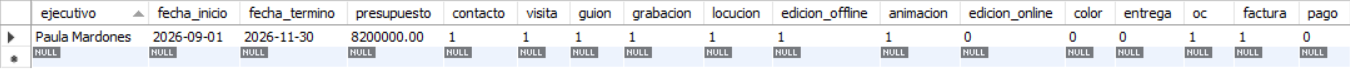
\includegraphics[width=\linewidth]{imagenes/image4.png}\captionof{figure}{Consulta 1: información general y avance del proyecto.}
\end{center}


\begin{center}
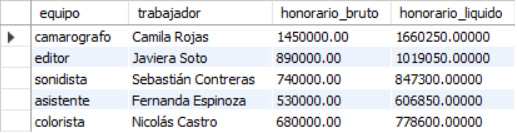
\includegraphics[width=0.87\linewidth]{imagenes/image5.png}\captionof{figure}{Consulta 1: trabajadores asignados y honorarios.}
\end{center}


\begin{center}
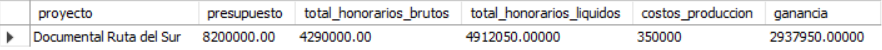
\includegraphics[width=\linewidth]{imagenes/image6.png}\captionof{figure}{Consulta 1: presupuesto y cálculo de la ganancia.}
\end{center}

Con los resultados de la primera consulta es posible observar el estado de un proyecto, las actividades ya realizadas, el equipo asociado y sus costos por honorarios, así como la ganancia que genera el proyecto en relación con los costos variables considerados.


\needspace{5\baselineskip}\subsubsection{Consulta 2: trabajadores y honorarios del período}

La segunda consulta genera una lista de los trabajadores que participaron en proyectos durante un mes y año específicos. Muestra la cantidad de proyectos en los que participó cada trabajador y los honorarios totales correspondientes al período. Se destaca dónde se seleccionan las fechas que deben modificarse según el período consultado:


\rotuloSQL{Código SQL: honorarios por trabajador y mes}
\begin{SQL}
USE mandalafilms;

SELECT
t.nombre_trabajador AS trabajador,
COUNT(DISTINCT(h.id_proyecto)) AS cantidad_proyectos,
SUM(h.honorario_bruto) AS total_honorarios_brutos,
(SUM(h.honorario_bruto)* 1.145) AS total_honrarios_liquidos
FROM trabajadores t
JOIN honorarios h ON t.id_trabajador = h.id_trabajador
JOIN proyectos p ON h.id_proyecto = p.id_proyecto
WHERE MONTH(p.fecha_termino) = '9' AND YEAR(p.fecha_termino) = '2026'
GROUP BY t.nombre_trabajador;
\end{SQL}

Esta consulta entrega el siguiente resultado:


\begin{center}
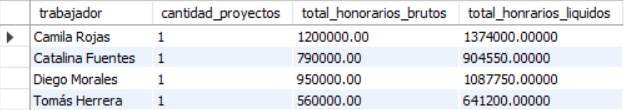
\includegraphics[width=0.92\linewidth]{imagenes/image7.png}\captionof{figure}{Consulta 2: honorarios por trabajador en el período seleccionado.}
\end{center}

Esta consulta muestra los trabajadores que estuvieron activos durante el mes, en cuántos proyectos participaron y cuánto se les paga en total durante ese período. Esto permite, además, llevar un registro de los gastos mensuales asociados a honorarios.


\needspace{5\baselineskip}\subsubsection{Consulta 3: ingresos, costos y resultado mensual}

La tercera y última consulta genera un consolidado de ingresos, gastos y resultados para un período específico. En este caso, nuevamente se deben ingresar manualmente los costos variables de producción, debido a su naturaleza particular para cada proyecto, como se explicó anteriormente. Se destacan los parámetros que deben modificarse según la consulta:


\rotuloSQL{Código SQL: consolidado de resultados mensuales}
\begin{SQL}
USE mandalafilms;

SET @costos_produccion_totales = 1500000.00;

Select
(SELECT SUM( p.presupuesto) FROM proyectos p
WHERE MONTH(p.fecha_termino) = 11 AND YEAR(p.fecha_termino) = 2026) AS ingresos,
SUM(h.honorario_bruto) AS honorarios_brutos_totales,
(SUM(h.honorario_bruto)*1.145) AS honorarios_liquidos_totales,
@costos_produccion_totales AS costos_produccion_totales,
ROUND((SUM(h.honorario_bruto)*1.145) + @costos_produccion_totales, 2) AS costos_variables_totales,
(SELECT SUM(costo) FROM costos_fijos) AS costos_fijos_totales,
ROUND( (SELECT SUM( p.presupuesto) FROM proyectos p WHERE MONTH(p.fecha_termino) = 11 AND YEAR(p.fecha_termino) = 2026) - ((SUM(h.honorario_bruto)*1.145) + @costos_produccion_totales) - (SELECT SUM(costo) FROM costos_fijos), 2) AS resultado_periodo
FROM honorarios h
JOIN proyectos p ON h.id_proyecto = p.id_proyecto
WHERE MONTH(p.fecha_termino) = 11 AND YEAR(p.fecha_termino) = 2026;
\end{SQL}

Esta consulta entrega el siguiente resultado:


\begin{center}

\includegraphics[width=\linewidth]{imagenes/image8.png}\captionof{figure}{Consulta 3: consolidado de ingresos, costos y resultado.}
\end{center}

Esta consulta ofrece una visión más completa del desempeño de la empresa durante un mes. Dado que se evalúa una cantidad reducida de proyectos, los costos resultan mayores que los ingresos dentro de la consulta. Esto no necesariamente indica una mala distribución de costos, sino que puede ser consecuencia de una simulación de datos muy acotada respecto de la operación real de la empresa, que puede desarrollar más de un proyecto audiovisual al mes para cubrir y justificar sus costos fijos.


\needspace{5\baselineskip}\section{Trazabilidad de la Entrega 1 a la Entrega 2}


\needspace{5\baselineskip}\subsection{Comparación de los cambios implementados}

La Entrega 2 incorpora cambios concretos respecto del diseño planteado en la Entrega 1. La tabla siguiente resume los principales ajustes implementados y su relación con lo definido inicialmente.


\begingroup
\footnotesize
\setlength{\tabcolsep}{3.0pt}
\renewcommand{\arraystretch}{1.17}
\begin{longtable}{|>{\RaggedRight\arraybackslash}p{0.155\linewidth}|>{\RaggedRight\arraybackslash}p{0.245\linewidth}|>{\RaggedRight\arraybackslash}p{0.3\linewidth}|>{\RaggedRight\arraybackslash}p{0.225\linewidth}|}
\hline
\rowcolor{grisTabla}
\textbf{Elemento} & \textbf{Entrega 1} & \textbf{Entrega 2} & \textbf{Motivo o evidencia} \\ \hline
\endfirsthead
\hline
\rowcolor{grisTabla}
\textbf{Elemento} & \textbf{Entrega 1} & \textbf{Entrega 2} & \textbf{Motivo o evidencia} \\ \hline
\endhead
\hline
\endfoot
Automatización & Se propuso una alerta de sobrecosto asociada al RF04. & Se implementó un flujo en n8n que recibe gastos, calcula el porcentaje ejecutado, clasifica el estado y genera alertas para los casos definidos. & Validar en la práctica la detección de gastos cercanos o superiores al presupuesto. \\ \hline
Cambios de etapa & Se definió que los avances debían confirmarse manualmente. & No se automatizaron los cambios de etapa. & Se mantuvo la decisión del dueño de ingresar manualmente los avances. \\ \hline
Modelo de datos & Se presentó un modelo ER preliminar con entidades, cardinalidades y PK candidatas. & Se desarrolló un modelo final normalizado a 3FN, con diccionario de datos, reglas de integridad, catálogos, vistas y nuevas restricciones. & Reducir redundancias, evitar inconsistencias y completar la implementación física del modelo. \\ \hline
Cliente & El atributo contacto reunía información de contacto en un mismo campo. & El atributo se separó en email y teléfono. & Cumplir 1FN y mantener atributos atómicos. \\ \hline
Proyecto & Guardaba \path{presupuesto_aprobado} y estado\_actual como atributos directos. & Se eliminó \path{presupuesto_aprobado} y el estado pasó a id\_etapa\_actual, relacionado con ETAPA. & Evitar duplicar el presupuesto de la cotización aprobada y eliminar texto libre en etapas. \\ \hline
Roles y asignaciones & Los roles se almacenaban como texto y se guardaba \path{honorario_calculado}. & Se agregó el catálogo ROL; el honorario se obtiene desde jornadas y tarifa pactada. & Evitar variantes de escritura y no almacenar valores derivados. \\ \hline
Hitos & La etapa y el estado se almacenaban directamente en HITO. & Se incorporó TIPO\_HITO, relacionado con ETAPA, y el estado se calcula a partir de las fechas. & Eliminar dependencias transitivas y apoyar la construcción de la Carta Gantt. \\ \hline
Gastos & GASTO almacenaba tipo y categoría. & Se creó CATEGORIA\_GASTO, que define el tipo, mientras GASTO conserva solo la referencia a la categoría. & Eliminar dependencia transitiva y conservar categorías aunque no existan gastos asociados. \\ \hline
Factura & Guardaba directamente el proyecto y el IVA. & Se eliminó id\_proyecto y el IVA se calcula desde el monto neto. & Evitar información redundante y posibles contradicciones con la OC. \\ \hline
Indicadores financieros & Se almacenaban valores como IVA, EBITDA y margen. & Se guardan los insumos históricos y los indicadores derivados se calculan mediante una vista. & Mantener una foto histórica sin almacenar datos derivados innecesarios. \\ \hline
Usuarios & No existía una entidad de usuarios en el ER preliminar. & Se agregó USUARIO. & Dar cobertura al requisito de autenticación RNF02. \\ \hline
Base de datos / SQL & Existía un modelo preliminar y no había consultas de negocio implementadas. & Se incorporaron datos sintéticos y consultas para proyectos, honorarios y resultados económicos. & Pasar desde el diseño conceptual a resultados que puedan ser consultados y analizados. \\ \hline
Datos de prueba & No existían datos sintéticos desarrollados para la ejecución de consultas. & Se generaron trabajadores, proyectos, asignaciones y costos ficticios. & Probar el funcionamiento sin publicar información privada real de la empresa. \\ \hline
\end{longtable}
\endgroup


\needspace{5\baselineskip}\section{Limitaciones y lecciones aprendidas}


\needspace{5\baselineskip}\subsection{Decisiones manuales y coherencia con el proceso}

Durante el desarrollo se observó que la automatización debe mantener coherencia con la forma real en que trabaja la empresa. No conviene automatizar todas las actividades. En este caso, los cambios de etapa y la evaluación del sobrecosto se mantuvieron como acciones manuales, respetando la decisión del dueño de conservar el control humano sobre el avance de los proyectos.


\needspace{5\baselineskip}\subsection{Pruebas y validación de datos}

Las pruebas realizadas en n8n también mostraron la importancia de validar los datos antes de utilizarlos en cálculos automáticos. Por ejemplo, cuando faltó el valor de gasto\_acumulado, el flujo generó un error NaN y se detuvo antes de registrar el caso. También se detectaron problemas con presupuestos iguales a cero, montos negativos y envíos simultáneos hacia Google Sheets. Estas pruebas permitieron corregir parte del flujo y demostrar que no basta con comprobar los casos normales: también es necesario probar entradas inválidas o incompletas.


\needspace{5\baselineskip}\subsection{Aspectos pendientes de integración}

Entre las principales limitaciones de la solución se encuentra que el flujo de n8n todavía simula la interacción con el SIG y no obtiene directamente desde la base de datos valores como el presupuesto aprobado o el gasto acumulado. Además, las notificaciones de sobrecosto se envían a webhook.site y el registro de las decisiones se realiza en Google Sheets, en lugar de integrarse directamente con Administración y Finanzas y con la base de datos del sistema. Los datos utilizados en las pruebas también son sintéticos.


\needspace{5\baselineskip}\subsection{Limitaciones del análisis SQL}

En la parte SQL, algunas consultas requieren ingresar manualmente valores asociados a los costos variables de producción, debido a que estos dependen de cada proyecto. Esto permite realizar las consultas y analizar los resultados, pero todavía limita la automatización completa del control de costos.


\end{document}
